\begin{frame}
    \begin{center}
        \Huge{Webanwendung}
    \end{center}
    \begin{figure}[h]
        \centering
        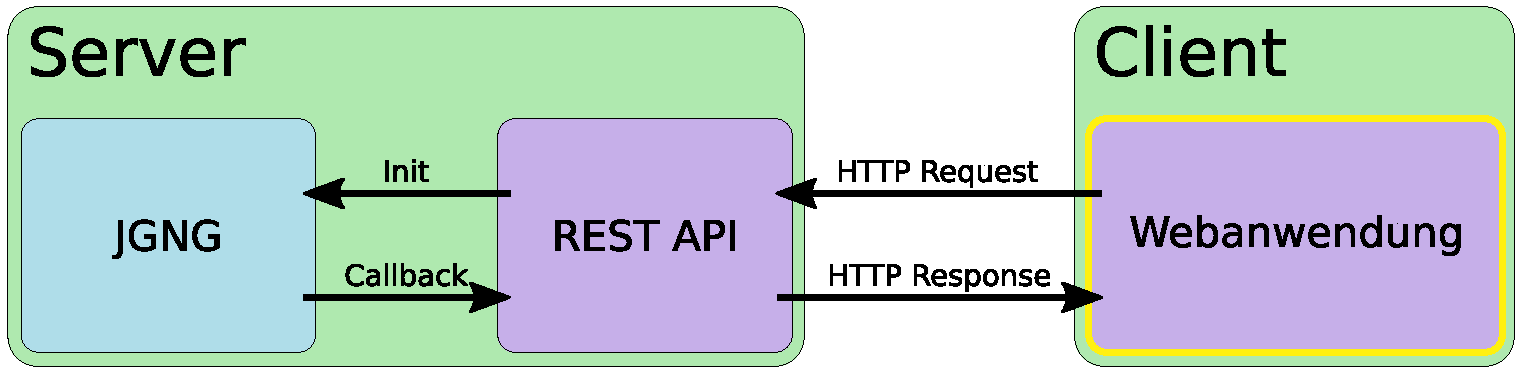
\includegraphics[width=\textwidth]{bilder/client-server_web-active.pdf}
    \end{figure}
\end{frame}
\subsubsection*{Layout und Umsetzung}
\begin{frame}
    \frametitle{Layout und Umsetzung}
    \begin{itemize}
        \item fixiertes Layout in der Aufteilung von 75\% (Graph) zu 25\% (Einstellungen) der Breite des Fensters
        \item Verwendung von \textbf{Bootstrap} (CSS) für die grundlegende Gestaltung
        \item Verwendung von \textbf{jQuery} (JS) zur Kommunikation mit der API mittels AJAX und JSON
        \item Verwendung des \textbf{Sigma} (JS) für die Darstellung des Graphen
    \end{itemize}
\end{frame}
\begin{frame}
    \frametitle{Ergebnis}
    \begin{figure}[h]
        \centering
        \includegraphics[width=0.9\textwidth]{../figures/jgng_net.png}
        %\caption{Webanwendung mit trainiertem JGNG}
    \end{figure}
\end{frame}
